% ------------------------------------------------------------------------ %
% !TEX encoding = UTF-8 Unicode
% !TEX TS-program = pdflatex
% !TEX root = ../Tesi.tex
% !TEX spellcheck = it-IT
% ------------------------------------------------------------------------ %
%
% ------------------------------------------------------------------------ %
% 	NOME CAPITOLO
% ------------------------------------------------------------------------ %
%
\chapter{Strumenti di sviluppo}
%
\label{cap:strumenti}
%
% ------------------------------------------------------------------------ %
%
\section{Introduzione}
%
L'applicazione che si vuole implementare è costituita da tre tipologie di entità: le prime corrispondo agli account dei \emph{medici} che hanno il compito di creare e rilasciare le ricette mediche bianche dematerializzate ai pazienti che le richiedono; le seconde sono i \emph{farmacisti} che hanno il compito di accertarsi che la ricetta dematerializzata non sia stata manomessa per procedere all'erogazione dei farmaci contenuti nella ricetta stessa; le terze sono gli account che, in questa implementazione, avranno il ruolo di \emph{amministratore} (admin) con la possibilità di associare un determinato ruolo (medico o farmacista) agli account esistenti.\\
Questo tipo di sistema può essere realizzato utilizzando come infrastruttura una blockchain privata: questa catena infatti contiene un insieme di transazioni attestanti ogni ricetta emessa dai medici e garantisce l'immutabilità del contenuto delle ricette stesse, permettendo i controlli di integrità sui contenuti inseriti. Inoltre la blockchain viene condivisa da tutte le parti coinvolte che, previo permesso, all'atto dell'ingresso nella rete possono scaricare localmente la copia più aggiornata e da quel momento in poi possono interagire con essa con nuovi inserimenti. Questa tecnologia infine rende immediatamente disponibili ogni inserimento di ricetta medica che viene trasmesso ad ogni nodo della rete. \\ 
Per una maggiore velocità nello sviluppo del prototipo applicativo, esso è stato pensato come un applicativo web. Generalmente, la struttura di una web application può essere schematizzata come nella seguente figura:
\begin{center}
	%
	\begin{figure}[H]
		%
		\centering
		%
		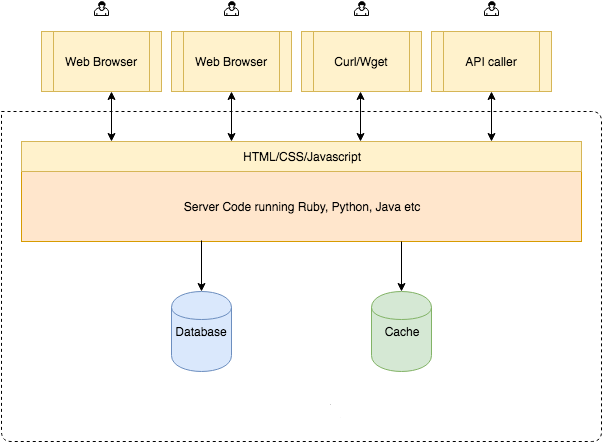
\includegraphics[width=.9\textwidth]{webapp}
		%
		\caption{Web application generica}
		%
		\label{fig:web application generica}
		%
	\end{figure}
	%
\end{center}
L'applicazione può essere ad esempio hostata su un servizio di hosting e tutti i client possono interagire con questa singola applicazione centrale. Un client può essere un browser oppure un'altra API che utilizza il servizio ecc. Quando il client effettua un richiesta al server quest ultimo prende in carico la richiesta, dialoga con il database e/o con la cache, legge/aggiorna/scrive il database\footnote{CRUD Model. Create, Read, Update, Delete} e serve il client. Questa tipologia di architettura è, al giorno d'oggi, una delle soluzioni tecniche più consolidate nell'ambito dello sviluppo del software. Però esistono anche determinate applicazioni dove sarebbe molto più utile se il database fosse ad esempio accessibile, in modo sicuro, da tutti senza dover dipendere da una terza parte. Questo è uno dei concetti chiave alla base di quelle che abbiamo definito precedentemente come \emph{Applicazioni decentralizzate} (Decentralized Application o Dapp). La struttura di una generica applicazione decentralizzata può essere invece schematizzata come segue:
\newline
%
\begin{center}
	%
	\begin{figure}[H]
		%
		\centering
		%
		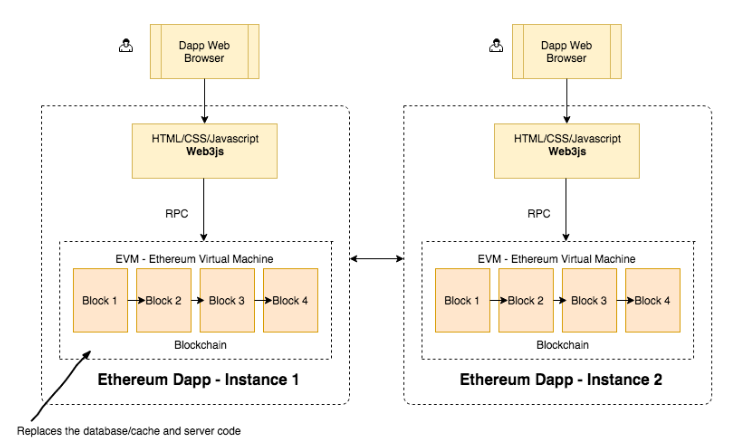
\includegraphics[width=.9\textwidth]{dapp}
		%
		\caption{Decentralized application generica}
		%
		\label{fig:decentralized application generica}
		%
	\end{figure}
	%
\end{center}
Possiamo vedere come il client (nel nostro caso il browser) comunica con la propria istanza dell'applicazione. Non c'è alcun server centrale al quale i client si connettono. Ogni elemento in figura rappresenta una scelta tecnologica relativa allo sviluppo della dapp. In particolare:
\begin{enumerate}
	\item i contratti sono scritti in \emph{Solidity}, linguaggio per scrivere Smart contract Ethereum che girano sulla EVM;
	\item \emph{Truffle} è uno dei framework più utilizzati a disposizione dello sviluppatore per lo sviluppo e il testing in ambiente Ethereum;
	\item \emph{Web3.js} è una Api Javascript per i client Ethereum che permette di comunicare con il nodo locale attraverso Remote Procedure Calls (RPC);
	\item la blockchain alla base della Dapp sarà Quorum.
\end{enumerate}
%
\section{Solidity}
Solidità è un linguaggio di alto livello \enquote*{contract-oriented} per l'implementazione di Smart Contract su varie piattaforme di Blockchain. È stato sviluppato da Gavin Wood ed è stato influenzato da C++, Python e JavaScript. Questo linguaggio viene compilato in bytecode eseguibile nell'Ethereum Virtual Machine (EVM) e supporta l'ereditarietà, le librerie e i tipi complessi definiti dall'utente. \\ 
Con Solidity, gli sviluppatori sono in grado di scrivere applicazioni che implementano una logica di business autodefinita ed integrata nello Smart contract, fornendo una transazione non ripudiabile ed autorevole. Come specificato da Wood, il linguaggio è progettato attorno alla sintassi \emph{ECMAScript} per renderlo familiare agli sviluppatori web ma, a differenza di ECMAScript, ha tipizzazione statica e tipi di ritorno variadici. Rispetto ad altri linguaggi attuali che vengono eseguiti su EVM come Serpent e Mutan, Solidity presenta delle differenze importanti:
\begin{itemize}
	\item sono supportate variabili membro complesse per contratti, incluse mappature e strutture arbitrariamente gerarchiche;
	\item è supportata l'ereditarietà, inclusa l'ereditarietà multipla con la linearizzazione C3;
	\item introduce una ABI che facilita funzioni multiple con la type-safety\footnote{la "sicurezza di tipo" è il modo con cui un linguaggio di programmazione previene o avvisa gli errori di tipo};
	\item è supportato da un sistema di documentazione che specifica una descrizione, di tipo user-centric, delle ramificazioni di una chiamata del metodo nota come \enquote*{Natural Language Specification}.
\end{itemize}%
Solidity inoltre ha a disposizione un ulteriore strumento molto potente per gli sviluppatori, chiamato \emph{Remix}, che consiste in un IDE Browser-based con integrato il compilatore e l'ambiente di runtime di Solidity senza componenti server-side. Le sue caratteristiche principali sono:
\begin{enumerate}
	\item sviluppo di smart contracts grazie all'editor integrato solidity;
	\item debug dell'esecuzione di uno smart contract;
	\item accesso allo stato e alle proprietà di uno smart contract già stato deployato;
	\item debug di transazioni che hanno già effettuato il commit;
	\item analisi del codice per minimizzare l'errore e per forzare le best practises.
\end{enumerate}
%
\begin{figure}[H]
	%
	\centering
	%
	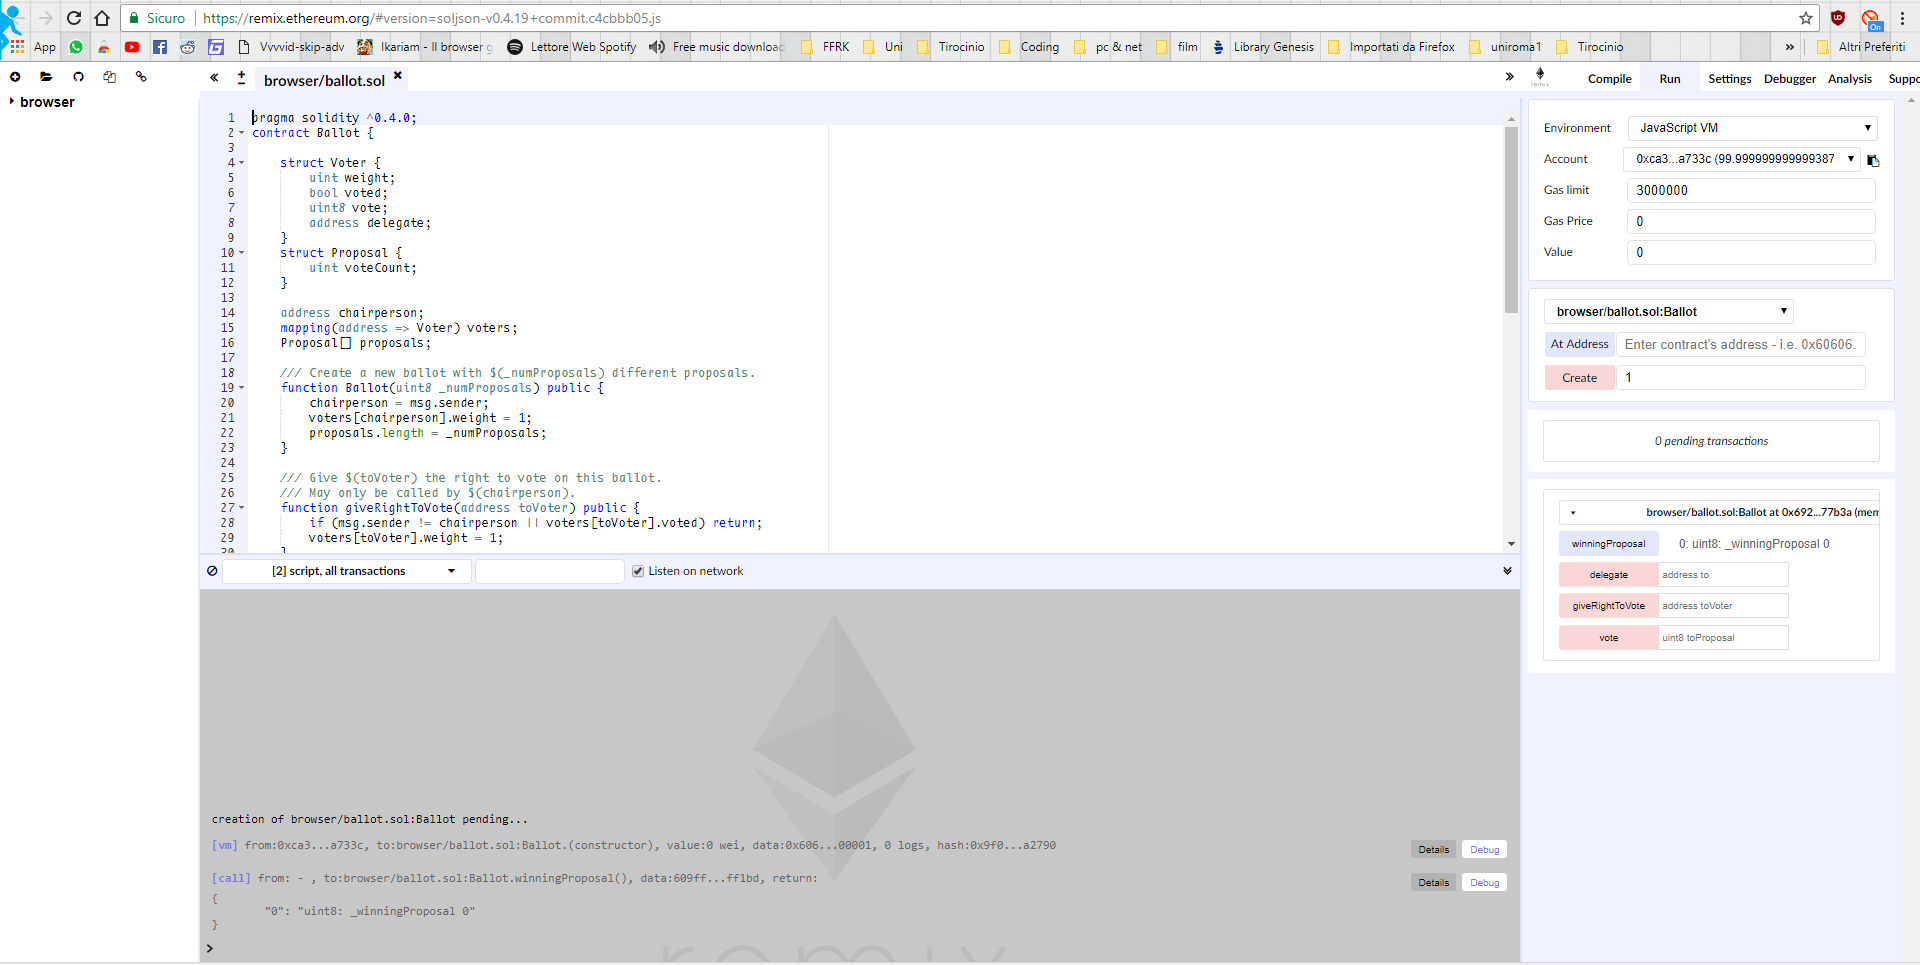
\includegraphics[width=.9\textwidth]{remix}
	%
	\caption{Remix IDE}
	%
	\label{fig:remix ide}
	%
\end{figure}
%
\section{Node.js \& Npm}%
\emph{Node.js} è un ambiente di run-time JavaScript, cross-platform e open-source per eseguire codice JavaScript lato server. Storicamente il linguaggio JavaScript è sempre stato principalmente usato come scripting lato client dove gli script erano integrati nelle pagine HTML per essere essere poi eseguiti dai motori JavaScript contenuti nei web browser degli utenti. Node.js permette al JavaScript di essere eseguito lato server per produrre pagine web dinamiche prima che esse vengano inviate al web browser dell'utente. Il modello di funzionamento di node è caratterizzato da un modello di I/O asincrono basato sugli eventi particolarmente adatto per le applicazioni web. La normale procedura di esecuzione di una applicazione server-side, scritta ad esempio in PHP, prevede lo scorrere di una serie di istruzioni che coinvolgono chiamate a servizi esterni come ad esempio query per un database, o l'accesso al filesystem per operazioni di lettura e scrittura. Tutti questi eventi sono bloccanti ovvero l'esecuzione dello script viene fermata finché non riceve una risposta dal componente esterno a cui l'ha richiesta. In tal modo il web server impiega la maggior parte del proprio tempo attendendo che i processi bloccati si completino, e questo porta ad una vistosa inefficienza nello sfruttamento delle risorse a disposizione. Tutto questo invece non succede in Node perchè, usando la programmazione asincrona, si elimina l'attesa e si eseguono le richieste successive, permettendo cosi un throughput e una scalabilità ottimizzate nelle web application. 
\subparagraph{Npm} è invece un gestore di pacchetti per il linguaggio JavaScript. In particolare è il gestore di pacchetti JavaScript predefinito nell'ambiente Node.js. Esso è composto da un client a riga di comando e da un database online di package pubblici (o moduli) denominato Npm registry. Un package è una directory che contiene uno o più file insieme ad un file chiamato package.json che contiene i dati relativi al pacchetto. Una web application che utilizza questa tecnologia per la gestione delle dipendenze in un progetto può contenere svariati pacchetti. Il vantaggio nell'usare un package manager risiede nella possibilità di aggiornare automaticamente tutte le dipendenze utilizzate evitando allo stesso tempo possibili "rotture" del codice causate da un aggiornamento manuale da parte dello sviluppatore. \\ 
Le tecnologie usate nello sviluppo dell'applicazione che si basano su Node.js sono:
\begin{itemize}
	\item Truffle framework;
	\item Express.js.
\end{itemize}
%
\subsection{Truffle Framework}
%
Truffle, attualmente, è il framework di sviluppo più popolare per applicazioni Ethereum based\footnote{Truffle supporta allo stesso modo la Blockchian Quorum essendo un fork di Ethereum}. Le feature che caratterizzano questo framework e che hanno portato alla sua scelta per lo sviluppo sono:
\begin{enumerate}
	\item \emph{Compilazione, linking, deployment e gestione dei binary degli smart contract integrata}. Il framework Truffle si occupa autonomamente della gestione degli artefatti dei contratti. Inoltre include il supporto per deploy custom, linking di librerie e applicazioni Ethereum complesse;
	\item \emph{Testing automatizzato dei contratti per un rapido sviluppo}. Truffle permette di scrivere test automatizzati sia in JavaScript che in Solidity per una maggiore rapidità di sviluppo;
	\item Permette di scrivere \emph{script di deploy custom} che riconoscono come l'applicazione possa cambiare nel tempo e che quindi permettono di avere uno sforzo di mantenimento minore;
	\item \emph{Gestione delle reti}. Truffle gestisce il deploy verso blockchain sia pubbliche che private. In questo modo lo sviluppatore non deve gestire manualmente gli artifatti di rete;
	\item Per utilizzare Truffle è necessario avere Node.js installato e questo permette di scaricare facilmente migliaia di dipendenze per gli Smart contracts via NPM;
	\item Truffle offre infine un ambiente ottimizzato nelle fasi di compilazione e test.
\end{enumerate}
Lo scheletro di un progetto Truffle è composto da quattro cartelle principali:
\begin{itemize}
	\item \emph{contracts/}: cartella dove sono contenuti i contratti Solidity.
	\item \emph{migrations/}: cartella dove sono contenuti gli scripts di migrazione.
	\item \emph{test/}: cartella dove sono contenuti i file per il test dell'applicazione e dei contratti.
	\item \emph{truffle.js}: file di configurazione di truffle.
\end{itemize}%
\subsection{Express.js}%
Express.js, o semplicemente Express, è un framework MVC per applicazioni web per Node.js, rilasciato come software libero ed open-source tramite MIT License ed è attualmente il framework server standard per Node.js. La filosofia di Express è quella di fornire un piccolo e robusto strumento per i server HTTP rendendolo la scelta preferita per le single page application, i siti web e le API. Come vedremo infatti, il compito principale di express all'interno del progetto sarà quello di gestire gli assett\footnote{I file statici come le viste} dell'applicazione e definire le rotte che saranno utilizzate per le richieste che arrivano dal client. Una rotta può essere una richiesta di tipo GET (semplice richiesta di file,passaggio di pochi parametri) e di tipo POST(passaggio di molti parametri con attivazione di logica lato server)
Nel nostro caso express ha in carico:
\begin{enumerate}
	\item gestione dei file statici dell'applicazione;
	\item la generazione del codice univoco NRE inserito nella ricetta dematerializzata ed utilizzato per la ricerca della ricetta stessa da parte dei farmacisti.
	\item la generazione server side del pdf della ricetta dematerializzata.
\end{enumerate}
La scelta di utilizzare di introdurre un elemento di tipo web server all'interno dell'architettura dell'applicazione è stata presa per motivi di sicurezza che saranno meglio spiegati durante la descrizione dell'implementazione dell'applicazione. 
%
\section{Web3.js} % 
Web3.js è una collezione di librerie scritte in JavaScript che permettono allo sviluppatore di interagire con un nodo locale o remoto di Ethereum/Quorum utilizzando una connessione HTTP o IPC. Web3 è necessaria affinche la dapp lavori con la blockchain in quanto fornisce lo strumento di comunicazione verso il nodo locale attraverso Remote Procedure Calls (RPC). In particolare, la libreria contiene un oggetto specifico per interagire con le blockchain Ethereum-based, l'oggetto \emph{web3.eth}. Per utilizzare la libreria, una volta importata nel progetto, si deve creare un'istanza di web3 andando a settare il provider per comunicare con il nodo locale:
\begin{lstlisting}[language=javascript]
	if (typeof web3 !== 'undefined') {
		web3 = new Web3(web3.currentProvider);
		} else {
		// set the provider you want from Web3.providers
		web3 = new Web3(new Web3.providers.HttpProvider("http://localhost:22000"));
	}
\end{lstlisting}%
A questo punto è possibile utilizzare le API dell'oggetto web3.
%
